\usetikzlibrary{calc}
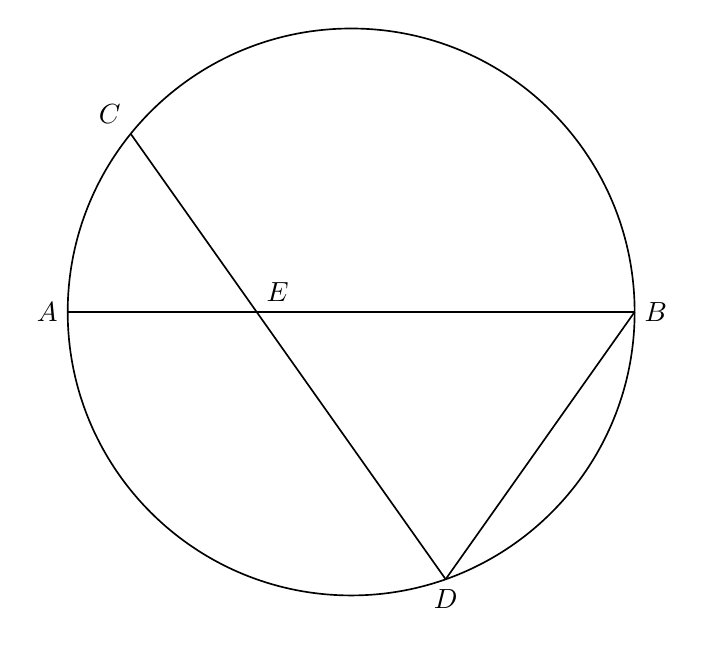
\begin{tikzpicture}[x=1cm,y=1cm,line width=.6pt,font=\normalsize]
\coordinate (O) at (1.2,0);
\coordinate (A) at (-2.4,0);
\coordinate (B) at (4.8,0);
\coordinate (E) at (0,0);
\coordinate (C) at (-1.6,2.2627);
\coordinate (D) at (2.4,-3.3941);
\draw (O) circle[radius=3.6cm];
\draw (A)--(B);
\draw (C)--(D);
\draw (B)--(D);
\node[left] at (A) {$A$};
\node[right] at (B) {$B$};
\node[above right] at (E) {$E$};
\node[above left] at (C) {$C$};
\node[below] at (D) {$D$};
\end{tikzpicture}
